\documentclass[10pt,twocolumn,letterpaper]{article}

\usepackage{cvpr}
\usepackage{times}
\usepackage{epsfig}
\usepackage{graphicx}
\usepackage{amsmath}
\usepackage{amssymb}
\usepackage{booktabs}

% Include other packages here, before hyperref.

% If you comment hyperref and then uncomment it, you should delete
% egpaper.aux before re-running latex.  (Or just hit 'q' on the first latex
% run, let it finish, and you should be clear).
\usepackage[breaklinks=true,bookmarks=false]{hyperref}

\cvprfinalcopy % *** Uncomment this line for the final submission

\def\cvprPaperID{****} % *** Enter the CVPR Paper ID here
\def\httilde{\mbox{\tt\raisebox{-.5ex}{\symbol{126}}}}

% Pages are numbered in submission mode, and unnumbered in camera-ready
%\ifcvprfinal\pagestyle{empty}\fi
\setcounter{page}{1}
\begin{document}

%%%%%%%%% TITLE
\title{Truth or DeGPTion: Evaluating Lie Detection Capabilities of GPT-3.5 through Fine-Tuning on Personal Opinions, Autobiographical Memories, and Intentions}


\author{
Tanner Graves\\
{\tt\small tanneraaron.graves@studenti.unipd.it}
\and
Marco Uderzo\\
{\tt\small marco.uderzo@studenti.unipd.it}
\and
Francesco Vo \\
{\tt\small francesco.vo@studenti.unipd.it}
\and
Mehran Faraji\\
{\tt\small mehran.faraji@studenti.unipd.it}
\and
Claudio Palmeri \\
{\tt\small claudio.palmeri@studenti.unipd.it}
% For a paper whose authors are all at the same institution,
% omit the following lines up until the closing ``}''.
% Additional authors and addresses can be added with ``\and'',
% just like the second author.
% To save space, use either the email address or home page, not both
}

\maketitle
%\thispagestyle{empty}


%%%%%%%%% ABSTRACT
\begin{abstract}
This paper aims at evaluating the capabilities of GPT3.5 in the task of Lie Detection.
This is done through the fine-tuning of GPT-3.5 on three English-language datasets encompassing 
personal opinions, autobiographical memories, and future intentions. 
Fine-tuning of LLMs consists in adapting a pre-trained language model to a specific 
task by further training the model on task-specific data, thereby 
enhancing its ability to generate contextually relevant and coherent text in 
line with the desired task objectives. In our investigation, the objective is to 
discern and classify instances of truth or deception.

\end{abstract}

%%%%%%%%% BODY TEXT
\section{Introduction}
Numerous academic publications consistently assert that the human capacity to discriminate 
between veracity and deception rests at chance-level proficiency. Consequently, an escalating 
interest has emerged in the application of machine learning (ML) methodologies, particularly 
those rooted in the Transformer Model, to enhance the accuracy of truthfulness prediction for statements. 
The intrinsic aptitude of ML models for pattern recognition empowers them to discern subtle cues 
that elude human perception. This research endeavors to employ OpenAI's GPT-3.5 Large Language Model (LLM) 
as the focal point, commencing with a comprehensive assessment of the base model's performance. Subsequently, 
an in-depth examination will be conducted on a fine-tuned GPT-3.5 model, specifically calibrated using the 
Personal Opinion Dataset (Deceptive Opinions), the Autobiographical Memories Dataset (Hippocorpus), and the 
Future Intention Dataset.

\subsection{Personal Opinion Dataset}

The participants of this study were divided in 4 groups (HIT’s) and asked to provide either 
a truthful or a deceptive opinion on the following topics: Abortion, Cannabis Legalization, Euthanasia, Gay Marriage, Policy on Migrants.
An extract from the table is shown below. \\

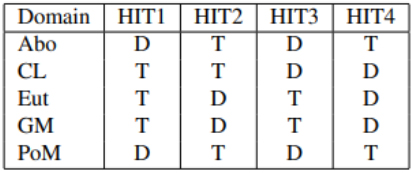
\includegraphics[scale=0.4]{img/pers_op_dataset.jpg}

\subsection{Autobiographical Memories Dataset}

This dataset contains 6854 diary-like short stories about salient life events gathered in 3 steps from 2 groups of people (A,B).
The study was conducted as following:

\begin{itemize}
    \item Stage 1: Group A writes 15-25 sentence truthful stories with a 2-3 sentence summary and a timeframe
    \item Stage 2: Group B is tasked to write an imaginative story with the summary of group A as a prompt
    \item Stage 3: After 2 months group A is asked to retell the story starting with their summary as a prompt
\end{itemize}
At the end a questionnaire was posed. \\

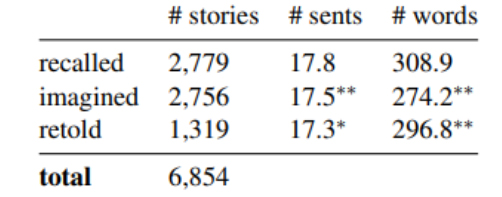
\includegraphics[scale=0.35]{img/autobio_mem_dataset.jpg}

\subsection{Future Intention Dataset}

The study from which this dataset was collected was conducted as following.

All participants are divided into either the truthful or deceptful group.
The former were asked to describe a non-work-related activity that would be doing in the next seven days answering the following questions:

\begin{itemize}
    \item Q1: “Please describe your activity as specific as possible”
    \item Q2: “Which information can you give us to reassure us that you are telling the truth”
\end{itemize}

The latter were given 3 activities from the former group, asked which ones didn’t apply to them and get 
randomly assigned one of those. After they were required to answer Q1, Q2 like the former group.
At the end a questionnaire was posed.

\section{Methods}

\subsection{Dataset Preprocessing}


The dataset was processed according to 'Scenario 3' of Loconte et al.\cite{Loconte}.
In Scenario 3, aggregation was performed on the three train and test sets from Scenario 1 (opinions, memories, intentions), followed by fine-tuning the model on the aggregated sets. 
This scenario evaluates the model's ability to classify truthful and deceptive statements across various contexts.

Regarding the implementation of this process, the single datasets were merged into a single one after being cleaned and shuffled. Then we divided it into training, validation and test set.
It is worth noting that we did not use all the data on the initial dataset, this is because the training of a LLM was made simpler by using a smaller training dataset.
Finally, the datasets were formatted into JSON to align with the expected input format of the OpenAI API. You can find the Python code in the \hyperref[sec:appendix]{Appendix} section of this paper.

In particular, the model was trained on two versions of the dataset:

\begin{itemize}
    \item a subset of the original dataset (Train: 210 examples; Validation: 45 examples; Test: 45 examples).
    \item the full dataset (Train: 6765 examples; Validation: 1450 examples; Test: 1450 examples).
\end{itemize}

\subsection{GPT-3.5 Fine-Tuning}
The model was trained utilizing the OpenAI API, and its performance was assessed through 
testing and comparison with GPT-3.5. Further experimentation was conducted to assess 
the impact of engineering the system prompt on overall performance.

Specifically, we noticed that the baseline GPT-3.5 prefers giving verbose or indecisive answers.
Verbose answers, that actually classify a statement as genuine or deceptive can be classified easily.
Nonetheless, the model decides not to give a definitive answer when it thinks it does not have enough information to classify the statement.
The following example shows this behaviour.

\begin{verbatim}
User: "Each and every abortion 
is essentially a tragedy. The 
potential mother will suffer 
unforeseen consequences. Society
as a whole will be deprived of 
the potential it could have 
received from the new life."

   
Baseline GPT-3.5: "There is no 
objective truth to the statement 
as it expresses subjective opinions
and beliefs about abortion. It cannot 
be definitively classified as 
'True' or 'False'."
\end{verbatim}   

To address this issue it was necessary to engineer a system prompt that
discourages this behaviour and adequately explains the task. This prompt
is provided to the model at every example query, so instructions should
be concise to minimize any token overhead that leads to increased cost of
training and queries.

\begin{verbatim}
System Prompt to Fine-Tuned GPT-3.5:

"You are an expert capable of
discerning truthful from deceptive
opinions based on speech patterns. 
Definitively classify the following 
statement as 'True' or 'False', 
based on the likelihood the statement
represents a genuinely held belief 
or a deception."
\end{verbatim}

This issue is avoided in the fine-tuned models as the training process
rewards our expected behaviour and output format.

The hyperparameters used for fine-tuning the model are declared in the table below. \\


\begin{tabular}{lcc}
    \toprule
    Model & Hyperparameter & Value \\
    \midrule
    Model 1 & Learning Rate & 0.001 \\
    & Epochs & 50 \\
    & Batch Size & 32 \\
    \midrule
    Model 2 & Learning Rate & 0.01 \\
    & Epochs & 30 \\
    & Batch Size & 64 \\
    \bottomrule
\end{tabular} \\

\subsection{Stylometric Analysis}

\section{Results}

\subsection{Lie Detection Task Performance}

Firstly, we evaluated the non-fine-tuned GPT-3.5 model, achieving 71.1\% accuracy.
After fine-tuning the 300 and 1500 model, we evaluated them in the same way.
Both the '300 Model' and '1500 Model' achieved 82.2\% accuracy, showing a considerable
improvement in performance. Moreover, the size difference in training example did not
affect the accuracy whatsoever, showing that fine-tuning on a smaller dataset is a good
option when training costs have to be minimized.

\subsection{Explainability Analysis (?)}

\section{Discussion}

Even though the baseline GPT-3.5 model is still capable of outperforming human capabilities, which
are at chance level, by a solid margin, the fine tuning process improves performance by 11.1\% in terms
of accuracy.

After examining the performance by class we found that the '1500 Model' performs poorly on the Future
Intentions Dataset, with a 69.7\% accuracy, which drags the overall performace down.

\section{Code Availability}
The datasets used and all the code used for this project is available
at the following \href{https://github.com/TannerAGraves/GPT-LieDetection/}{GitHub Repository}.


%-------------------------------------------------------------------------


{\small
\bibliographystyle{ieee_fullname}
\bibliography{egbib}
}

\clearpage % Start a new page
\onecolumn % Switch to one-column layout

\section{Appendix}
\label{sec:appendix}

\subsection{Python Code}

The following code preprocesses the dataset according to Scenario 3.
The original Python Notebook is located at the following \href{https://colab.research.google.com/github/TannerAGraves/GPT-LieDetection/blob/main/dataset/datasets.ipynb}{link} in our GitHub Repository

\begin{verbatim}
import numpy as np
import pandas as pd
from sklearn.model_selection import train_test_split

dc = pd.read_csv('DecOp_data_EN_500.csv', sep=',', encoding='UTF-8')

d1 = []
for i in range(dc.shape[0]):
  row = dc.iloc[i]
  d1.append({'ID': row['ID'],
      'age' :row['age'], 'gender': row['gender'],
  'sent' : row['A'].replace('\n', " ") ,
  'labels'  : row['GT.A']})

  d1.append({'ID': row['ID'],
      'age' :row['age'], 'gender': row['gender'],
  'sent' : row['E'].replace('\n', " ")  ,
  'labels'  : row['GT.E']})
  d1.append({'ID': row['ID'],
      'age' :row['age'], 'gender': row['gender'],
  'sent' : row['GM'].replace('\n', " ")  ,
  'labels'  : row['GT.GM']})

  d1.append({'ID': row['ID'],
      'age' :row['age'], 'gender': row['gender'],
  'sent' : row['Pom'].replace('\n', " ")  ,
  'labels'  : row['GT.Pom']})

  d1.append({'ID': row['ID'],
      'age' :row['age'], 'gender': row['gender'],
  'sent' : row['CL'].replace('\n', " ")  ,
  'labels'  : row['GT.CL']})

decop = pd.DataFrame.from_records(d1)

decop = decop[['ID', 'sent', 'labels']]
decop['type'] = 'A'

decop

hc = pd.read_csv('hcV3-stories.csv', sep=',', encoding='UTF-8')

mem = hc[hc['memType']!='retold']
mem = mem.dropna(subset=['story', 'memType'])
mem = mem[['story', 'memType']]
mem['memType'][mem['memType']=='recalled'] = 'T'
mem['memType'][mem['memType']=='imagined'] = 'F'
mem = mem.rename(columns={'story': 'sent', 'memType': 'labels'})
mem['type'] = 'B'

mem

intent = pd.read_csv('sign_events_data_statements.csv', encoding="UTF-8")

intent.loc[intent['outcome_class']=='t', 'outcome_class'] = 'T'
intent.loc[intent['outcome_class']=='d', 'outcome_class'] = 'F'
intent['q1'] = intent['q1'].apply(lambda x: x.replace('\n', ''))
intent = intent.rename(columns={'q1': 'sent', 'outcome_class': 'labels'})
intent = intent[['sent', 'labels']]
intent['type'] = 'C'

intent

k = 300
seed = 42

'''
shuffled_df = decop.sample(frac=0.1, random_state=seed).copy()
sample_decop = shuffled_df.iloc[:k,].copy()
sample_decop.drop('ID', axis=1, inplace=True)
sample_decop

data = pd.concat([sample_decop, mem.iloc[:k,].copy(), intent.iloc[:k,].copy()],
                 ignore_index=True)
'''

decop.drop('ID', axis=1, inplace=True)

data = pd.concat([decop, mem, intent], ignore_index=True)
data_shuffle = data.sample(frac=1, random_state=seed+27).reset_index(drop=True)
data_shuffle['labels'] = data_shuffle['labels'].map({'T': 1, 'F': 0})
data_shuffle.rename(columns={'sent': 'text', 'labels': 'label', 'type': 'set'}, 
                                                                        inplace=True)

data_shuffle = data_shuffle.iloc[:k,]

train_data, temp_data = train_test_split(data_shuffle, test_size=0.3, random_state=42)

val_data, test_data = train_test_split(temp_data, test_size=0.5, random_state=42)

train_data.to_json(f'train_data_{k}.json', orient='records', lines=True)

val_data.to_json(f'val_data_{k}.json', orient='records', lines=True)

test_data.to_json(f'test_data_{k}_class.json', orient='records', lines=True)

data_shuffle.shape

train_data.shape
\end{verbatim}

\end{document}
